\section{Definizione di Progetto}
\subsection{Project Management Body of Knowledge}
Non esiste una sola definizione di progetto. Diamo diverse definizioni perché servono per esprimere un punto di vista. Nel caso del Project Management sono molto più importanti le opinioni che le definizioni. Vi sono varie sfumature di pensiero che i professionisti hanno sul tema. Ci sono tuttavia definizioni più importanti, come quella del \textbf{Project Management Body of Knowledge (PMBOK)}, che è uno standard di fatto. Uno standard è un documento formale che descrive delle norme, dei metodi, dei processi e delle pratiche consolidate. Per creare uno standard serve un'associazione di professionisti, una comunità internazionale che certifichi cosa davvero può essere preso come riferimento.\newline
La guida PMBOX fornisce delle buone linee guida ma il mondo è variegato e non ci sono indicazioni molto specifiche.\newline
PMBOK nasce per gestire il singolo progetto, l'iterazione tra più progetti richiede più lavoro. Anche questo corso è focalizzato sul singolo progetto.\newline
PMBOK non è l'unico standard. PMBOK nasce per i progetti tradizionali (la struttura dei processi è a cascata). Per il momento ci concentriamo su questo standard. Una possibile alternativa è PRINCE2 (più orientato sulle metodologie). Ci sono numerose anche numerose proposte Agile (Scrum, Kanban, etc.).\newline\newline
Nella guida di PMBOK con "corpo di conoscenze" si intende una raccolta di conoscenze dei Project Manager che hanno raccolto esperienze e ogni tanto apportano modifiche alle edizioni che escono.\newline
Esistono alcune keyword importanti che vengono utilizzate in un certo modo:
\begin{itemize}
	\item \textbf{Generalmente riconosciuto}: significa che i project manager sono sostanzialmente d'accordo su un punto. C'è un forte consenso.
	\item \textbf{Buona prassi}: una buona pratica è un suggerimento su come fare qualcosa che si è assodato essere una buona soluzione.
\end{itemize}
La guida PMBOK fornisce e promuove un vocabolario comune nell'ambito professionale. Alcuni termini sono utilizzati nelle riunioni ed indicano qualcosa di ben definito che è difficile capire se si è esterni al contesto aziendale.\newline
\subsection{Definizione di progetto}
Segue la definizione di progetto secondo PMBOK, e la definizione di altri elementi utili per approfondire:
\begin{itemize}
	\item \textbf{Progetto (secondo PMBOK)}: un'iniziativa \textcolor{red}{temporanea} intrapresa per creare un prodotto, un servizio o un altro risultato con caratteristiche di \textcolor{red}{unicità}.
	\begin{info}
		Il risultato del progetto non è solo l'applicazione, ma tutto ciò che ne consegue. Prodotto e servizio in ambito informatico hanno una linea di demarcazione molto fine.\newline
		La keyword \textcolor{red}{temporanea} è importante perché implica che il progetto ha un inizio e una fine. I motivi sono molteplici. Si rischia di non avere un riferimento temporale per poi non convergere. Non avendo una fine si rischia che il cliente aggiunge nuove funzionalità di continuo. A non essere temporanea è il risultato (es: la torre Eiffel), o meglio, lo è ma deve avere una durata abbastanza ampia.\newline
		La keyword \textcolor{red}{unicità} invece è importante perché un risultato unico è molto più richiesto e necessario di qualcosa che già esiste.\newline
	\end{info}
	\item \textbf{Attività}: La descrizione di un pezzo di lavoro che rappresenta uno step in un processo. L'attività può essere sia un workflow sia manuale.
	\begin{info}
		L'attività di Workflow richiede un'iterazione uomo-macchina.
	\end{info}
	\item \textbf{Attività operativa}: è un impegno di lavoro continuo, solitamente è un processo ripetitivo che segue le procedure esistenti in un'organizzazione. I processi aziendali sono predefiniti e non cambiano mai. Un'azienda seria dovrebbe avere la documentazione che descrive come vanno eseguiti i processi aziendali. Se i processi non sono formalizzati e sono solo nelle menti delle persone le informazioni vanno ovviamente disperse.\newline\newline
	L'attività di definire come deve funzionare un processo aziendale è unica o ripetitiva? Si tratta a tutti gli effetti di un progetto. Non è importante che il progetto sia grande, l'importante è che abbia un inizio, una fine, e che sia unico.
	\begin{warn}
		Un progetto NON è un'attività operativa.
	\end{warn}
	\item\textbf{Attività di progetto}: lavoro che deve essere svolto, ha caratteristiche di unicità ed è inserito in un processo unico e specifico per ogni progetto. Non è da confondersi con un'attività operativa. Ha un overhead, perché essendo unica non è mai stata fatta prima e quindi va gestita nel modo corretto. Necessario anche stimare il tempo che può richiedere, dato che a differenza di un'attività operativa la durata non è ben nota.
	\begin{info}[Esempio - Differenza tra progetto ed attività operativa]
		Vogliamo realizzare un nuovo ristorante, la cucina, il servizio di prenotazione, il take-away etc.\newline
		Servono dei processi aziendali \textit{(attività operative)} per raccogliere ordini, preparare portate, consegnare ordini, gestire prenotazioni etc.\newline
		Le attività operative iniziano nel momento in cui apre il ristorante.\newline
		Il menù a quale categoria appartiene? Se l'attività operativa o progettuale? Dipende, se il menù è fisso e i piatti sono a rotazione in base al periodo dell'anno o ad altro allora si tratta di attività operativa. Se invece magari il piatto del giorno non è prefissato da nessuna parte allora stiamo già parlando di un progetto (guarda caso è un piatto unico).\newline
		Esistono approcci che combinano le attività operative e di progetto, come nel caso di \textbf{DevOps}.
	\end{info}
	\item \textbf{Progetto (Wysocki)}: una sequenza unica, complessa e connessa di attività che hanno un obiettivo che devono essere completate rispettando le specifiche e i vincoli di tempo e di budget.
	\begin{info}
		In questo caso l'unicità del progetto si sposta sull'unicità delle attività. Le attività hanno dipendenze tra loro. Bisogna pensare a quali attività vengono prima di altre e alle interrelazioni che le attività hanno tra loro.
	\end{info}
	\item \textbf{Business value}: Anche detto valore di business, indica un valore che deve dare vantaggi tangibili all'azienda nelle sue attività di business. Si tratta del valore "percepito" dal destinatario del prodotto o servizio creato dal progetto.
	\begin{info}
		In questa visione un progetto è una sequenza finita di attività dipendenti tra loro, il cui completamento con successo si traduce nella fornitura del "business value" atteso. Nelle nostre soluzioni prioritizzeremo e daremo più importanza alle attività che massimizzano il business value.
	\end{info}
\end{itemize}
Un progetto può creare:
\begin{itemize}
	\item \textbf{Un prodotto} finito, un componente di un altro prodotto...
	\item \textbf{Un servizio} o ciò che serve per effettuarlo, ad esempio il modo in cui svolgere assistenza ai clienti.
	\item \textbf{Una versione migliorata di un prodotto o di un servizio} già esistente. Si riducono i difetti e si aggiungono funzionalità.
	\item \textbf{Conoscenza}, ad esempio un progetto di ricerca per risolvere un problema in un nuovo modo.
	\item Altro...
\end{itemize}
I progetti sono spesso utilizzati come mezzo per realizzare/concretizzare il piano strategico di un'organizzazione. Le considerazioni strategiche che possono portare all'autorizzazione di un progetto sono molteplici: richiesta del mercato, richiesta del cliente, progresso tecnologico, requisiti legali etc.
\subsection{Definizione di programma}
Un \textit{Programma} è un insieme di progetti correlati gestiti in modo coordinato. Il fine è ottenere benefici e un controllo che non sarebbe possibile gestendo individualmente i singoli progetti.\newline
I progetti infatti
\begin{itemize}
	\item contribuiscono ad uno stesso obiettivo, che può essere molto articolato;
	\item hanno punti di iterazione, anche piuttosto forti. Spesso persone diverse lavorano su progetti diversi;
	\item spesso i budget sono in comune tra i progetti;
\end{itemize}
Spesso i progetti di un programma creano dei componenti utili per il raggiungimento di un risultato finale.\newline
Definiamo come \textbf{Program Management} la gestione centralizzata e coordinata dei progetti di un programma, al fine di raggiungere obiettivi e benefici strategici. Il focus e sulle interdipendenze dei progetti, tra queste vi sono:
\begin{itemize}
	\item \textbf{Risoluzione di vincoli legati a risorse e/o conflitti}: risolvendo un vincolo che colpisce più progetti risolviamo un problema che è più "pesante" (risorse, budget etc...).
	\item \textbf{Allineare la direzione organizzativa e/o strategica}: un ripensamento in un progetto può avere impatti molto pesanti su tutto il programma.
	\item \textbf{Risolvere questioni relative alla gestione del cambiamento}: ad esempio rivedere un intero processo in funzione di un cambiamento desiderato o non.
\end{itemize}
Si parla di \textbf{Programma} quando abbiamo forti interrelazioni tra i progetti. Nel caso in cui le interrelazioni invece sono deboli conviene parlare di \textbf{Portfolio}.
\subsection{Definizione di portfolio}
Un \textbf{Portfolio} è un insieme di progetti che vengono raggruppati solo per facilitare la gestione efficace ed efficiente del lavoro complessivo. Ad esempio può aver senso aggregare i progetti gestiti da una singola business unit, ad un gruppo di ricerca a progetti con lo stesso budget etc.\newline
\centeredImage{document/img/projectportfolioprogram.PNG}{Relazione tra progetto, portfolio e programma secondo PMBOK}{0.9}
\subsection{Scope (ambito) del progetto}
Lo scope (o ambito) definisce i confini del progetto in termini di ciò che deve essere fatto e ciò che non deve essere fatto.\newline
Molto importante è avere una prioritizzazione dei requisiti di progetto e degli obiettivi.\newline
Un primo problema è mappare subito lo scope con le specifiche funzionali, ma lo scope sta ad un livello molto più alto. Una modalità di specificare i requisiti denominata RBS (decomposizione ad albero) ci mostrerà che in alto ci sono i goals mentre molto più in basso appunto le specifiche funzionali. Il punto dello scope è mostrare anche le specifiche non funzionali.\newline
Lo scope rappresenta il concetto che dobbiamo mantenere integro. Importante è usare il tempo iniziale nel progetto per definire in modo chiaro lo scope. L'esito può essere:
\begin{itemize}
	\item è tutto molto chiaro;
	\item pensiamo di aver capito l'ambito, ma non siamo sicuri al 100\% (un esempio è il caso della ricerca e dello sviluppo, in cui si pensa di avere una buona soluzione ma bisogna fare ulteriori accertamenti);
\end{itemize}
Lo scope è un ottimo strumento anche per capire quanta incertezza sui requisiti c'è riguardo il progetto.\newline
Anche lo scope può essere soggetto al cambiamento.
\subsection{Qualità}
Come giudichiamo un prodotto di qualità? Ci sono diversi indici a cui possiamo pensare:
\begin{itemize}
	\item Corretto Funzionamento;
	\item Accessibilità e facilità d'utilizzo;
	\item Efficienza;
	\item Buon Design;
	\item Molto altro...
\end{itemize}
In un progetto vengono considerati due tipi di qualità:
\begin{itemize}
	\item \textbf{Qualità del prodotto}: riferito al deliverable;
	\item \textbf{Qualità del processo}: riferita al processo di getsione del progetto;
\end{itemize}
La qualità è importante perché permette di garantire la soddisfazione del cliente e permette di utilizzare meglio le risorse, permettendo di risparmiare tempo e denaro.
\subsection{Ciclo di vita del progetto (PMLC)}
Non abbiamo una definizione formale, il ciclo di vita è tutto ciò che accade da quando inizia e finisce un progetto. La stessa cosa può essere detta del ciclo di vita di un prodotto.
\centeredImage{document/img/cycle.PNG}{Sequenza delle fasi in un ciclo di vita del progetto}{0.4}
\begin{itemize}
	\item \textbf{Idea}: nasce l'idea per il progetto;
	\item \textbf{Charter}:documento su cui si lavora sugli obiettivi;
	\item \textbf{Gruppo Project Management}: formazione di un team che si occupi del PM.
	\item \textbf{Descrizione dell'ambito}: si descrive l'ambito del progetto (esistono casi in cui conviene fermare un progetto in questa fase, perché magari troppo rischioso o dispendioso, o il "business value" è marginale).
	\item \textbf{Piano}: una volta definiti i requisiti si traducono in un piano e quindi in un attività che poi ci porterà ad avere un prezzo. In questa fase possiamo capire che un'idea interessante può essere troppo onerosa da portare avanti;
	\item \textbf{Baseline}: Inizia la parte in cui non si può sbagliare, acquisire risorse è costose e i rischi sono di far fallire il progetto.
	\item \textbf{Avanzamento}: si inizia con l'implementazione, coi test etc.
	\item \textbf{Accettazione}: si arriva alla fine del progetto in uno stato che si crede accettabile.
	\item \textbf{Approvazione}: da parte del cliente;
	\item \textbf{Consegna}: presso il cliente;
\end{itemize}
Ci saranno anche ovviamente attività di revisione o di aggiornamento. Possiamo vedere queste attività come dei piccoli progetti, dato che verranno rilasciati risultati.
\centeredImage{document/img/costolivello.PNG}{Costo e livello del personale tipico nel ciclo di vita di un progetto}{0.5}
\noindent Effettuare modifiche in una fase iniziale costa molto poco. Apportare modifiche verso la fine del progetto significa buttare via del lavoro svolto.
\centeredImage{document/img/influenzastake.PNG}{Influenza dei stakeholder nel corso del tempo}{0.5}
\subsection{Scope Triangle}

Immaginiamo di avere un triangolo i cui lati sono \textbf{Tempo}, \textbf{Costi} e \textbf{Risorse disponibili}. La lunghezza del lato dipende dalla quantità disponibile del relativo soggetto. L'area invece è lo scope, cioè ciò che vogliamo mettere in un progetto. Non avendo budget tempo e risorse possiamo immaginare di avere un triangolo con poca area.\newline
La possibilità di aumentare i lati del triangolo e di conseguenza aumentare l'area a volte c'è. L'alternativa è potare i requisiti o reinserirli in un progetto futuro. Anche la qualità è negoziabile, per questo fa parte dell'area del triangolo come lo scope.
\begin{figure}[H]
	\centering
	\begin{subfigure}{.3\textwidth}
		\centering
		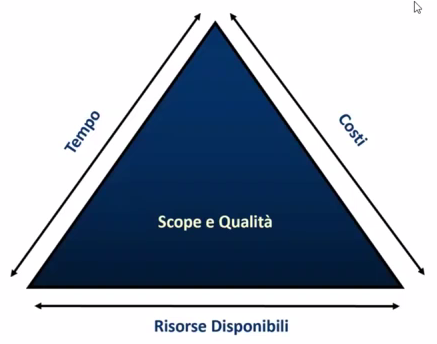
\includegraphics[width=\linewidth]{document/img/triangle.PNG}
		\caption{Scope triangle v.1}
	\end{subfigure}%
	\begin{subfigure}{.3\textwidth}
		\centering
		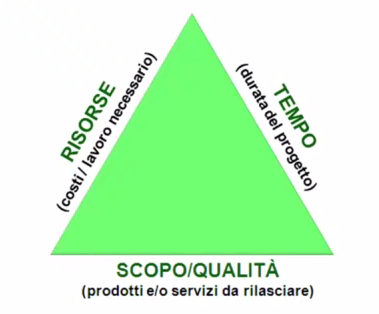
\includegraphics[width=\linewidth]{document/img/triangle2.PNG}
		\caption{Scope triangle v.2}
	\end{subfigure}%
	\begin{subfigure}{.3\textwidth}
		\centering
		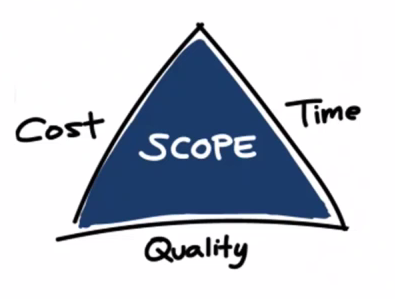
\includegraphics[width=\linewidth]{document/img/triangle3.PNG}
		\caption{Scope triangle v.3}
	\end{subfigure}
\end{figure}

\noindent Ci sono tanti altri tipi di triangoli, nessuno è corretto, sbagliato o meglio degli altri. L'importante è ricordarsi di questa metafora per ricordarsi di tutte quante le disponibilità. Secondo Wysocki non tutte le variabili hanno la stessa priorità:
\centeredImage{document/img/table.PNG}{Variabile con priorità secondo Wysocki}{0.5}
\noindent L'importante è mantenere in equilibrio il triangolo. Una modifica delle variabili può destabilizzare il progetto. Quando questo accade bisogna riportare in equilibrio il triangolo.
\begin{info}[Esempio]
	Se siamo in ritardo il lato del triangolo relativo al tempo è diventato più corto, e quindi dobbiamo aumentare budget o risorse.
\end{info}
\subsubsection{Problem Escalation Strategy}
La domanda che ci permette di porre lo scope triangle è "a chi appartiene cosa?"\newline
Nel caso in cui ci serva più tempo per esempio il "cosa" è il tempo. A chi appartiene il tempo. Al team del progetto, al cliente, al senior management...
Nel migliore dei casi si riesce a creare una nuova organizzazione all'interno del team e si riesce a recuperare tempo. Nel caso in cui il team non riesca il project manager può cercare di riallocare risorse o budget. Nel caso peggiore può essere necessario chiedere al cliente più tempo, che può essere disposto o non disposto a darcelo in base ai suoi bisogni, il suo umore, o da come è stato redatto il contratto. Nel caso in cui si arrivi a contrattare col cliente è importante ri-negoziare su più aspetti: tempo, budget, scope.
\subsection{Creeps : definizione e gestione}
Le creeps sono quei cambiamenti lievi ed impercettibili ed insidiosi, ma quando i loro effetti si accumulano possono diventare problemi importanti.
\begin{itemize}
	\item \textbf{Scope Creep}: Avviene perché delle condizioni esterne cambiano, per esempio quando esce una nuova tecnologia che surclasssa la soluzione che stiamo mettendo in atto. Questa viene classificata come creep perché tutti i lievi ma impercettibili cambiamenti in ciò che ci circonda può portare a violare l'integrità concettuale di ciò che stiamo sviluppando. Per ovviare a questa creep è necessario capire appieno cosa comporta ogni decisione presa in corso d'opera;
	\item \textbf{Hope Creep}: Un comportamento individuale da monitorare con attenzione. Si tratta di una situazione in cui per esempio si perde del tempo e si nasconde una situazione critica perché si è convinti di poter recuperare nei giorni successivi. Solitamente non si riesce a recuperare e la situazione può peggiorare. Portato avanti da più persone il tempo perso è notevole. Recuperare tempo attraverso straordinari aumenta i costi.
	\item \textbf{Effort Creep}: Questa Creep è abbastanza vaga nella sua definizione. Nonostante l'effort non si riesce ad arrivare al risultato sperato, nonostante tutto sembri andare per il verso giusto, per esempio se la percentuale delle attività compiute è del 95\% resta invariata nel giro di una settimana. Questo può essere dovuto all'errato monitoraggio dell'attività, la scarsa organizzazione del lavoro, l'inesperienza etc.
	\item \textbf{Feature Creep}: Riguarda un comportamento scorretto di un membbro del team, anche se è abbastanza legato allo Scope Creep. Questa creep riguarda l'aggiunta di funzionalità non concordate con il cliente, il project manager e l'architetto. Il dev aggiunge feature credendo che possa essere utile all'utente ma spesso non è così. Se il cliente non ha chiesto la funzionalità c'è un motivo, si aggiunge complessità e si perde tempo. Questa creep è evitabile solo grazie all'audit, ossia dei check di qualità.\newline
	Se un membro del team è convinto una feature sia assolutamente necessaria deve richiedere l'autorizzazione per aggiungerla. La richiesta seguirà un iter definito dal project manager. L'autorizzazione deve essere concessa:
	\begin{itemize}
		\item dal projetc manager per quanto riguarda gli aspetti gestionali;
		\item dall'architetto per ciò che riguarda aspetti architetturali;
		\item dal cliente, che deve riconoscere il valore della feature.
	\end{itemize}
\end{itemize}
\subsection{Classificare i progetti}
Non tutti i processi devono essere implementati allo stesso modo per tutti i progetti. Serve una classificazione per i progetti, che è possibile:
\begin{itemize}
	\item Per \textbf{dimensione} (costi, durata etc.)
	\item Per \textbf{applicazione} (sviluppo software, installazione etc.)
	\item Per \textbf{tipo} (nuovo, manutenzione, etc.). Alcuni esempi sono lo svilupo di un'app, l'installazione di hw o sw, l'aggiornamento delle procedure aziendali...
	\item In base alla \textbf{complessità} o al livello di \textbf{incertezza}.
	\item Si può classificare un progetto rispetto a determinate \textbf{caratteristiche}:
	\begin{itemize}
		\item rischio;
		\item business value;
		\item durata;
		\item complessità;
		\item tecnologia impiegata;
		\item numero di reparti impegnati;
		\item costi.
	\end{itemize}
\end{itemize}
